\documentclass[11pt,a4paper]{article}
\usepackage{paquete}


\begin{document}


\pagestyle{fancy}
%\renewcommand{\sectionmark}[1]{\markboth{}{\thesection\ \ #1}}
\lhead{\sc }
\chead{}
\rhead{\rightmark}
\lfoot{}
\cfoot{}
\rfoot{\thepage}

%\begin{comment}
%
% Carátula:

\begin{titlepage}

\thispagestyle{empty}

\begin{center}

\includegraphics[scale=0.5]{./figuras/logo_utn}\\
\hfill \newline
\large{\textsc{Resumen Paradigma Funcional}}\\
\large{\textsc{Facultad Regional Buenos Aires}}\\
\large{\textsc{Universidad Tecnologica Nacional}}\\
\end{center}

% \newline
\begin{center}
\LARGE{\textsc{Paradigmas de Programación -- $K2032$}}\\
\hfill \newline
\huge{Trabajos Prácticos}
\end{center}

\vspace{2cm}



\begin{center}
	\begin{tabular}{lc}
		PAZ PORTILLA, José Miguel & \ \ \ 2028244 \\
		\texttt{\href{mailto:jpazportilla@frba.utn.edu.ar}{jpazportilla@frba.utn.edu.ar}}\\
	\end{tabular}
\end{center}

\vspace{1cm}
\begin{center}
\large{\today}
\end{center}

\end{titlepage}

%
% Pongo el índice en una página aparte:
%
{
  \hypersetup{linkcolor=black}
  \tableofcontents
}
% \tableofcontents
\thispagestyle{empty}
\newpage
%
% Hago que las páginas se comiencen a contar a partir de aquí:
%
\setcounter{page}{1}



\newpage
%%%%%%%%%%%%%%%%%%%%%%%%%%%%%%%%%%%%%%%%%%%%%%%%%%%%%%%%%%%%%%%%%%%%%%%

\section{Introducción a Objetivo}
En este paradigma de objetos se vuelve a tener efecto, pero es menos declarativo que funcional y lógico. Se utiliza el lenguaje de programación Wollok. La idea es combinar estructuras de datos y operaciones.

Las caracteristicas de un objeto son:

\begin{enumerate}
	\item Exponen una interfaz, es un conjunto de operaciones con las que se pueden interactuar con el objetos. Solo se puede interactuar con objetos mediantes mensajes. Los mensajes que un objeto entiende va a ser el resultado de poseer metodos.
	\item Pueden llegar a tener estado interno, que son atributos, es decir referencias a otros objetos. Estos atributos pueden cambiar de referencia y apuntar a otros objetos.
	\item Tienen una identidad, cada objeto es diferente a cualquier otro, aunque hayan otros que respondan a los mismos mensajes y estado interno.
\end{enumerate}

\subsection{Problema: La Golondrina Pepita}

\begin{itemize}
	\item Un ornitólogo nos pide ayuda para estudiar el Consumo de Energía de la golondrina Pepita
	\item El Volar consume energia de Pepita.
	\item El Comer recupera la energía de Pepita.
\end{itemize}

\subsubsection{Resolución: La Golondrina Pepita}
\begin{itemize}
	\item La palabra object define un objeto nuevo.
	\item La palabra var define un atributo que podrá ser cambiado
	\item La palabra method permite crear métodos.
	\item El metodo volar() y comer() causan efecto.
	\item El metodo energia() son solo de consulta.
\end{itemize}

\subsubsection{Wollok: La Golondrina Pepita}
\lstinputlisting[language=java]{codigos/video17_e1_pepita/src/pepita.wlk}

\subsection{Problema: La entrenadora de aves Emilia}
\begin{itemize}
	\item Emilia solo sabe entrenar aves
	\item La aves deben comer 5g, volar 10km y volver a comer 5g.
\end{itemize}

\subsubsection{Resolución: La entrenadora de aves Emilia}
\begin{itemize}
	\item Emilia no conoce a Pepita, pero como Pepita entiende los mensajes come y vola, entonces podra entrenarla.
\end{itemize}

\subsubsection{Wollok: La entrenadora de aves Emilia}
\lstinputlisting[language=java]{codigos/video17_e1_pepita/src/emilia.wlk}

\subsection{Emilia entrena a Pepita}
Emilia puede entrenar a cualquier objeto que entienda los mensajes come y vola. En la \autoref{fig:test emilia entrena a pepita} se observa que pepita sufre el efecto luego que emilia la entrena, aumentando su energia de $100J$ a $180J$.


\subsubsection{Wollok:Emilia entrena a Pepita}
\lstinputlisting[language=java]{codigos/video17_e1_pepita/src/test.wtest}

\begin{figure}[H]
	\centering
	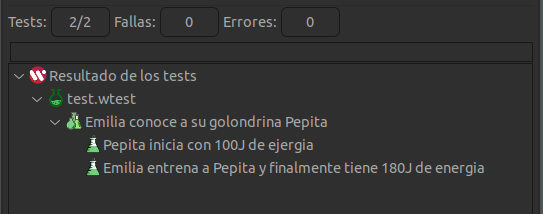
\includegraphics[scale=0.7]{figuras/test_pepita_emilia.png}
    \caption{Test unitario de pepita siendo entrenada por emilia.}
    \label{fig:test emilia entrena a pepita}
\end{figure}  

\subsection{Conceptos clave de la programación orientada a objetos}

%%%%%%%%%%%%%%%%%%%%%%%%%%%%%%%%%%%%%%%%%%%%%%%%%%%%%%%%%%%%%%%%%%%% 
\newpage

\appendix
\section{Apéndice}
%\lstinputlisting[]{codigos/video17_e1_pepita/src/pepita.wlk}
%\lstinputlisting{codigo.asm}

\end{document}
